\chapter{Random variables, expectation, and variance}

\section{Random variables}

A {\it random variable} (r.v.) is defined on a probability space $(\Omega, \pr)$ and 
is a mapping from $\Omega$ to $\R$. 

The value of the random variable is fully determined by the outcome $\omega \in \Omega$.
Thus the underlying probability space (probabilities $\pr(\omega)$) induces a probability
distribution over the random variable. Let's look at some examples.

Suppose you roll a fair die. The sample space is $\Omega = \{1,2,3,4,5,6\}$, all outcomes 
being equally likely. On this space we can then define a random variable
$$ X = \left\{ \begin{array}{ll}
               1 & \mbox{if die is $\geq 3$} \\
               0 & \mbox{otherwise}
               \end{array} \right.$$
In other words, the outcomes $\omega = 1,2$ map to $X = 0$, while the outcomes 
$\omega = 3,4,5,6$ map to $X = 1$. The r.v. $X$ takes on values $\{0,1\}$, with 
probabilities $\pr(X = 0) = 1/3$ and $\pr(X=1) = 2/3$.

Or say you roll this same die $n$ times, so that the sample space is 
$\Omega = \{1,2,3,4,5,6\}^n$. Examples of random variables on this larger space are
\begin{eqnarray*}
X & = & \mbox{the number of 6's rolled,} \\
Y & = & \mbox{the number of 1's seen before the first 6.}
\end{eqnarray*}
The sample point $\omega = (1,1,1,1,\ldots,1,6)$, for instance, would map to 
$X = 1, Y = n-1$. The variable $X$ takes values in $\{0,1,2,\ldots,n\}$,
with
$$ \pr(X = k) 
\ = \ 
{n \choose k} \left(\frac{1}{6} \right)^k \left( \frac{5}{6} \right)^{n-k} $$
(do you see why?).

As a third example, suppose you throw a dart at a dartboard of radius $1$, and that it
lands at a random location on the board. Define random variable $X$ to be the distance
of the dart from the center of the board. Now $X$ takes values in $[0,1]$, and for 
any $x$ in this range, $\pr(X \leq x) = x^2$.

Henceforth, we'll follow the convention of using capital letters for r.v.'s.




\section{Finite, Infinite, and Undefined Expectations}
% Akshay: I believe this should actually go after the definition of expected value a couple of sections below, but am writing it here anyway.

In this section, we'll only look at integer-valued random variables. 
We will see that such \emph{discrete} random variables can have an expectation (mean) 
that is finite, infinite, or even undefined!

For these purposes, we'll need to recall a few specific series discussed earlier: 
the geometric series
$$ \sum_{i=1}^\infty \frac{1}{2^i} = 1 $$
the finite series
$$ \sum_{i=1}^\infty \frac{1}{i^2} = \frac{\pi^2}{6} $$
and the infinite \emph{harmonic series}
$$ \sum_{i=1}^\infty \frac{1}{i} $$

\subsection{Finite Expectation}
It's not news to us that a discrete random variable can have finite expectation, 
thanks to the familiar examples of a coin flip or dice roll. 
We should note that even if a random variable can take on infinitely many values, it can have a finite expectation.
An example is the number of coin flips up to and including the first ``heads," as we've seen.


\subsection{Infinite Expectation}
It's also possible for a valid random variable to have an infinite expectation. 
For example, consider a random variable $X$ over the positive integers $\{1, 2, 3, \dots\}$, 
such that $\pr(X = i) = \frac{6}{\pi^2 i^2}$. 
This is clearly a valid distribution as seen earlier, because $ \frac{6}{\pi^2} \sum_{i=1}^\infty \frac{1}{i^2} = 1 $. 

However, the expectation of $X$ is
$$ \sum_{i=1}^\infty i \cdot \pr(X = i) = \sum_{i=1}^\infty \frac{6}{\pi^2 i} = \frac{6}{\pi^2} \sum_{i=1}^\infty \frac{1}{i} $$
which, as we recognize from above, is a multiple of the \emph{infinite} harmonic series. 

What does it mean to have an infinite expected value? 
Well, suppose we divided the rotating wheel into a countably infinite number of slices, 
so that segment $i$ takes up a fraction $\frac{6}{\pi^2 i^2}$ of the wheel. 
If the wheel is spun as before, and a ticket pays us $\$i$ for landing on slice $i$, 
then what we've shown above is that our mean payout from any spin is infinite. 
In other words, we should be willing to pay any (finite) price for the ticket, no matter how high, 
because we'd always expect to receive more money in return.


\subsection{Undefined Expectation}
We've seen that finite and infinite expected values are possible for a discrete random variable. 
Interestingly, there is a third possibility - that the expected value is undefined. 
In this case, it's impossible to pin down a single value for the random variable's mean!

To give an example, consider a random variable $X$ over the nonzero integers $\mathbb{Z} \setminus \{0\} = \{\dots, -3, -2, -1, 1, 2, 3, \dots\}$, 
such that 
$$\pr(X = i) = \begin{cases} \frac{6}{\pi^2 i^2} & i \text{ is odd and } i > 0 \\ \frac{6}{\pi^2 i^2} & i \text{ is even and } i < 0 \\ 0 & \text{otherwise} \end{cases} $$

First, we check that it's a valid distribution: 
$$ \sum_{i \in \mathbb{Z} \setminus \{0\}} \pr(X = i)
= \frac{6}{\pi^2} \left( \sum_{i \in \{ 1, 3, 5, \dots \}} \frac{1}{i^2} + \sum_{i \in \{\dots, -6, -4, -2 \}} \frac{1}{i^2} \right) 
= \frac{6}{\pi^2} \left( \frac{\pi^2}{6} \right) = 1 $$

But what's the expected value of $X$? 
Using the definition of expectation, it's 
\begin{align*}
\sum_{i \in \mathbb{Z} \setminus \{0\}} i \cdot \pr(X = i) 
&= \frac{6}{\pi^2} \left( \sum_{i \in \{ 1, 3, 5, \dots \}} \frac{1}{i} + \sum_{i \in \{\dots, -6, -4, -2 \}} \frac{1}{i} \right) \\
&= 1 - \frac{1}{2} + \frac{1}{3} - \frac{1}{4} + \frac{1}{5} - \dots \\
&= \left( 1 - \frac{1}{2} - \frac{1}{4} \right) + \left( \frac{1}{3} - \frac{1}{6} - \frac{1}{8} \right) + \left( \frac{1}{5} - \frac{1}{10} - \frac{1}{12} \right) + \dots \\
&= \left( 1 - \frac{1}{2} - \frac{1}{4} \right) + \left( \frac{1}{3} - \frac{1}{6} - \frac{1}{8} \right) + \left( \frac{1}{5} - \frac{1}{10} - \frac{1}{12} \right) + \dots
\end{align*}

So the sum is equal to half of itself? 
This appears quite strange, and it turns out that through similar rearrangements of the sum, we can make it evaluate to any real number we choose. 
This is why we don't even try to define a specific value for the sum, and instead call the expected value of $X$ \emph{undefined} in this case.

What does this mean? 
Going back to the example of the wheel and the ticket to spin it, we are saying that there is no fixed fair price for the ticket. 
Under these circumstances, we're best advised to avoid playing the game at all.

Incidentally, the rearrangement trick we've played above is very dependent on there being positive and negative terms in the sequence. 
We might ask whether it's possible to do this when there are only positive terms in the sequence. 
The answer is no - for a random variable that doesn't take negative values, this ``undefined" strangeness cannot occur. 

It turns out that if $\sum_k |a_k|$ is finite for any sequence $a_k$ (known as \emph{absolutely convergent}), then this kind of thing won't happen. 
(Note that this isn't the case here, because $\sum_k |a_k|$ is the infinite harmonic series.)

%(For those interested, there's more. Mention Riemann rearrangement theorem in English?)



\section{Arithmetic and Geometric Series}

The simplest {\it arithmetic series} is $1,2,3,\ldots$. The sum of the first 
$n$ elements of this series is
$$ 1 + 2 + \cdots + n \ = \ \frac{n(n+1)}{2} .$$

Why? suppose that write the sum twice, first going up from $1$ to $n$
and then and then going down from $n$ down to $1$:
$$ \left(1 + 2 + \cdots + (n-1) + n\right) + 
\left(n + (n-1) + \cdots + 2 + 1\right) $$
We can rearrange the sum into a sum of $n$ pairs, the first of which
sums the first element in each list, the second sums the second
elements in each list etc:
$$ (1+n) + (2+(n-1)) + (3+(n-2)) + \cdots + (n+1) $$
It is easy to see that each pair sums to $n+1$ and that there are $n$
pairs, which gives a total of $n(n+1)$. Recalling that we summed two
copies of the original sum we get $n(n+1)/2$.

A more general arithmetic series is $a, a+s, a+2s, \ldots$
(where $a,s$ are some numbers). The sum of the first $n$ elements of this series is
$$ a + (a+s) + \cdots + (a + (n-1)s)
\ = \ 
an + s(1 + \cdots + (n-1))
\ = \ 
an + \frac{sn(n-1)}{2}.
$$
\\

One of the most common {\it geometric series} is $1, 2, 4, 8, \ldots$; the sum
of the first $n$ elements of this series is
$$ 1 + 2 + \cdots + 2^{n-1} \ = \ 2^n - 1 .$$
Another common series is $1, \frac{1}{2}, \frac{1}{4}, \ldots$,
in which the first $n$ terms sum to $2 - (1/2^{n-1})$.

More generally, a geometric series is of the form $a, ar, ar^2, ar^3, \ldots$
(where $a,r$ are some numbers), and its first $n$ terms sum to
$$ a + ar + \cdots + ar^{n-1} 
\ = \ 
\frac{a(r^n-1)}{r-1}
\ = \ 
\frac{a(1-r^n)}{1-r}.$$
The first form is more useful when $r > 1$, while the second is more useful when $r< 1$.

In the case where $|r| < 1$, we can sum the entire series (with infinitely many terms) 
to get $a/(1-r)$.

\section{The mean, or expected value}

For a random variable $X$ that takes on a finite set of possible values, the 
{\it mean}, or {\it expected value}, is
$$ \E(X) \ = \ \sum_{x} x \, \pr(X = x) $$
(where the summation is over all the possible values $x$ that $X$ can have). This
is a direct generalization of the notion of {\it average} (which is typically
defined in situations where the outcomes are equally likely). If $X$ is a continuous 
random variable, then this summation needs to be replaced by an equivalent integral; 
but we'll get to that later in the course.

Here are some examples.
\begin{enumerate}
\item {\it Coin with bias (heads probability) $p$.}

Define $X$ to be $1$ if the outcome is heads, or $0$ if it is tails. Then 
$$ \E(X) 
\ = \ 
0 \cdot \pr(X = 0) + 1 \cdot \pr(X = 1)  
\ = \ 
0 \cdot (1-p) + 1 \cdot p
\ = \ 
p .
$$

Another random variable on this space is $X^2$, which also takes on values in $\{0,1\}$.
Notice that $X^2 = X$, and in fact $X^k = X$ for all $k = 1,2,3,\ldots$! Thus, 
$\E(X^2) = p$ as well. This simple case shows that in general, $\E(X^2) \neq \E(X)^2$.

\item {\it Fair die.}

Define $X$ to be the outcome of the roll, so $X \in \{1,2,3,4,5,6\}$. Then
$$ \E(X) 
\ = \ 
1 \cdot \frac{1}{6} + 2 \cdot \frac{1}{6} + 3 \cdot \frac{1}{6} + 4 \cdot \frac{1}{6}
+ 5 \cdot \frac{1}{6} + 6 \cdot \frac{1}{6} 
\ = \ 
3.5.$$

\item {\it Two dice.}

Let $X$ be their sum, so that $X \in \{2,3,4,\ldots, 12\}$. We can calculate the probabilities
of each possible value of $X$ and tabulate them as follows:

\begin{center}
\begin{tabular}{c|c|c|c|c|c|c|c|c|c|c|c}
$x$          & 2 & 3 & 4 & 5 & 6 & 7 & 8 & 9 & 10 & 11 & 12 \\ \hline
$\pr(X = x)$ & $\frac{1}{36}$ & $\frac{2}{36}$ & $\frac{3}{36}$ & $\frac{4}{36}$ & $\frac{5}{36}$ & $\frac{6}{36}$ & $\frac{5}{36}$ & $\frac{4}{36}$ & $\frac{3}{36}$ & $\frac{2}{36}$ & $\frac{1}{36}$  
\end{tabular}
\end{center}

This gives $\E(X) = 7$.

\item {\it Roll n die; how many sixes appear?}

Let $X$ be the number of $6$'s. We've already analyzed the distribution of $X$, so
$$ E(X) 
\ = \ 
\sum_{k = 0}^n k \, \pr(X = k)
\ = \ 
\sum_{k = 0}^n k {n \choose k} \left(\frac{1}{6} \right)^k \left( \frac{5}{6} \right)^{n-k}
\ = \ 
\frac{n}{6}.
$$
The last step is somewhat mysterious; just take our word for it, and we'll get back to it later!

\item {\it Toss a fair coin forever; how many tosses to the first heads?}

Let $X \in \{1,2,\ldots\}$ be the number of tosses until you first see heads. Then
$$ \pr(X = k)
\ = \ 
\pr((T,T,T,\ldots,T,H))
\ = \ 
\frac{1}{2^k}.
$$
It follows that 
$$ \E(X) 
\ = \ 
\sum_{k=1}^\infty \frac{k}{2^k} 
\ = \ 
2.
$$
We saw in class how to do this summation. The technique was based on the formula for the
sum of a geometric series: if $|r| < 1$, then
$$ a + ar + ar^2 + \cdots \ = \ \frac{a}{1-r}.$$

\item {\it Toss a coin with bias $p$ forever; how many tosses to the first heads?}

Once again, $X \in \{1,2,\ldots\}$, but this time the distribution is different:
$$ \pr(X = k)
\ = \ 
\pr((T,T,T,\ldots,T,H))
\ = \ 
(1-p)^{k-1}p.
$$
Using the same technique as before, we get $\E(X) = 1/p$.

There's another way to derive this expectation. We always need at least one coin toss.
If we're lucky (with probability $p$), we're done; otherwise (with probability $1-p$),
we start again from scratch. Therefore $\E(X) = 1 + (1-p) \E(X)$, so that $\E(X) = 1/p$.

\item {\it Pascal's wager: does God exist?}

Here was Pascal's take on the issue of God's existence: if you believe there is
some chance $p > 0$ (no matter how small) that God exists, then you should behave
as if God exists.

Why? Well, let the random variable $X$ denote your amount of suffering.

Suppose you behave as if God exists (that is, you are good). This behavior incurs
a significant but finite amount of suffering (you are not able to do some of the
things you would like to). Say $X = 10$.

On the other hand, suppose you behave as if God doesn't exist -- that is, you 
do all the things you want to do. If God really doesn't exist, you're fine, and 
your suffering is $X = 0$. But if God exists, then you go straight to hell
and your suffering is $X = \infty$. Thus your {\it expected} suffering
if you behave badly is $\E(X) = 0 \cdot (1-p) + \infty \cdot p = \infty$.

So: to minimize your expected suffering, behave as if God exists!

\end{enumerate}


\subsection{An application to sampling}

Suppose you are interested in finding out the fraction of Americans who like sushi. 
This is some unknown value $p \in [0,1]$ that you decide to estimate by sampling.
To this end, you pick $n$ random people and poll them. Let $X_i$ be $1$ if the $i$th
person you ask likes sushi, and $0$ if not. Your estimate of $p$ is then
$$ Y \ = \ \frac{X_1 + \cdots + X_n}{n}.$$

Since $\E(X_i) = p$, it follows by linearity of expectation that
$$
\E(Y)
\ = \ 
\frac{1}{n} \left( \E(X_1) + \cdots + \E(X_n) \right)
\ = \ 
p.
$$
So $Y$ certainly has the right expected value. But how far does it typically
deviate from this expectation? Since the $X_i$ are independent, and since
each $\var(X_i) = p(1-p)$ (recall our earlier coin flip example), 
$$ 
\var(Y) 
\ = \ 
\frac{\var(X_1 + \cdots + X_n)}{n^2}
\ = \ 
\frac{\var(X_1) + \cdots + \var(X_n)}{n^2}  
\ = \ 
\frac{p(1-p)}{n}.
$$
So the standard deviation of $Y$ is $\sqrt{p(1-p)/n}$: the larger $n$ is,
the closer $Y$ stays to the desired value $p$.

\section{Linearity of expectation}

If you double each value of $X$, then you also double its average; that is, 
$\E(2X) = 2 \E(X)$. Likewise, if you raise each of its values by 1, you will
also increase the average by 1; that is, $\E(X+1) = \E(X) + 1$. More generally,
for any constants $a,b$,
$$ \E(aX + b) \ = \ a\E(X) + b.$$
Another exceptionally useful formula says that the mean value of the sum of
variables is simply the sum of their individual means. Formally, for 
any random variables $X, Y$,
$$ \E(X+Y) \ = \ \E(X) + \E(Y).$$
For example, recall our earlier example about two
rolls of a die, in which we let $X$ be the sum of the rolls and derived $\E(X)$
by first computing $\pr(X = x)$ for all $x \in \{2,3,\ldots,12\}$. Well, now
we can do it much more easily: simply write $X_1$ for the first roll and $X_2$
for the second roll, so that $X = X_1 + X_2$. We already know $\E(X_i) = 3.5$,
so $\E(X) = 7$.

More generally, for any random variables $X_1, X_2, \ldots, X_n$,
$$ \E(X_1 + \cdots + X_n) \ = \ \E(X_1) + \cdots + \E(X_n) .$$
Some quick examples:
\begin{enumerate}
\item Roll $n$ dice and let $X$ be the number of sixes. What is $\E(X)$?

This time, let $X_i$ be $1$ if the $i$th roll is a six, and $0$ otherwise. Thus 
$\E(X_i) = 1/6$, so $\E(X) = n/6$.

\item Toss $n$ coins of bias $p$ and let $X$ be the number of heads. What is $\E(X)$?

Let $X_i$ be $1$ if the $i$th coin turns up heads, and $0$ if it turns up tails. Then
$\E(X_i) = p$ and since $X = X_1 + \cdots + X_n$, we have $\E(X) = np$.

\item Toss $n$ coins of bias $p$; what is the expected number of times $HTH$ appears 
in the resulting sequence?

Let $X_i$ be $1$ if there is an occurrence of $HTH$ starting at position $i$ (so
$1 \leq i \leq n-2$). The total number of such occurrences is
$X = X_1 + X_2 + \cdots + X_{n-2}$. Since $\E(X_i) = p^2(1-p)$, we have 
$\E(X) = (n-2) p^2(1-p)$.
\end{enumerate}

\subsection{Fixed points of a permutation}

The {\it fixed points} of a permutation are the numbers that remain in their original 
position. For instance, in the permutation
$$ (1,2,3,4,5,6) \rightarrow (6,2,5,4,1,3)$$
the fixed points are 2 and 4. Let $X$ be the number of fixed points in a random 
permutation of $(1,2,\ldots, n)$; what is $\E(X)$?

Linearity is very helpful here. Define the random variable $X_i$ to be $1$ if $i$
is a fixed point, and $0$ otherwise. Then $\E(X_i) = 1/n$. Therefore
$$ \E(X) 
\ = \ 
\E(X_1 + \cdots + X_n)
\ = \ 
1.
$$
The expected number of fixed points is 1, regardless of $n$.

\subsection{Coupon collector, again}

Recall the setting: each cereal box holds one of $k$ action figures (chosen at random), and
you want to collect all the figures. What is the expected number of cereal boxes you need
to buy?

Suppose you keep buying boxes until you get all the figures. Let $X_i$ be the number of 
boxes you buy to get from $i-1$ distinct figures to $i$ distinct figures. Therefore
$X = X_1 + X_2 + \cdots + X_k$, and of course $X_1 = 1$.

What is $\E(X_i)$? Well, you already have $i-1$ of the figures, so the chance of getting
a new figure in a cereal box is $(k-(i-1))/k$. Call this $p$. Therefore, the expected amount 
of time you have to wait to get a new figure is $1/p$: just like waiting for a coin with
bias $p$ to turn up heads. That is,
$$ \E(X_i) \ = \ \frac{k}{k-i+1} .$$

Invoking linearity of expectation,
\begin{eqnarray*}
\E(X) & = & \E(X_1) + \cdots + \E(X_k) \\
      & = & \frac{k}{k} + \frac{k}{k-1} + \frac{k}{k-2} + \cdots + \frac{k}{1} \\
      & = & k \left( 1 + \frac{1}{2} + \cdots + \frac{1}{k} \right) \\
      & \approx & k \ln k.
\end{eqnarray*}
This confirms our earlier observations about the coupon collector problem: you need
to buy about $k \ln k$ boxes.

\subsection{Balls in bins, again}

Toss $m$ balls in $n$ bins; what is the expected number of {\it collisions}? Let's make
this more precise. For any $1 \leq i < j \leq m$, define the random variable $X_{ij}$ to
be $1$ if balls $i$ and $j$ land in the same bin, and $0$ otherwise. Then the
number of collisions is defined to be
$$ X  \ = \ \sum_{1 \leq i < j \leq m} X_{ij} .$$

Since $\E(X_{ij}) = 1/n$ (do you see why?), it follows that the expected number of 
collisions is 
$$ \E(X) \ = \ {m \choose 2} \frac{1}{n} \ = \ \frac{m(m-1)}{2n} .$$
So if $m < \sqrt{2n}$, the expected number of collisions is $< 1$, which means
every ball goes into a different bin. 

This relates back to the birthday paradox, where $m$ is close to the threshold $\sqrt{2n}$.

\section{Independent random variables}

Random variables $X$ and $Y$ are {\it independent} if
$$ \pr(X=x, Y=y) \ = \ \pr(X=x) \pr(Y=y) $$
for all $x,y$. In words, the joint distribution of $(X,Y)$ factors into the product
of the individual distributions. This also implies, for instance, that
$$ \pr(X = x | Y = y) \ = \ \pr(X=x) .$$

Which of the following pairs $(X,Y)$ are independent?
\begin{enumerate}
\item Pick a random card out of a standard deck. Define $X$ to be $1$ if it is a heart;
 and $0$ otherwise. Define $Y$ to be 1 if it is a jack, queen, or king; and $0$ otherwise.
\item Toss a fair coin $n$ times, and define $X$ to be the number of heads, and $Y$ to 
be $1$ if the last toss is heads (and $0$ otherwise).
\item $X$ and $Y$ take values in $\{-1,0,1\}$, and their joint distribution is given by 
the following table of probabilities.

\begin{center}
\begin{tabular}{|cc|ccc|} \hline
\multicolumn{2}{|c|}{} & \multicolumn{3}{c|}{Y} \\ 
\multicolumn{2}{|c|}{}        & $-1$   & $0$    & $1$ \\ \hline
\multirow{3}{*}{X}     & $-1$ & $0.4$  & $0.16$ & $0.24$ \\ 
                       & $0$  & $0.05$ & $0.02$ & $0.03$ \\ 
                       & $1$  & $0.05$ & $0.02$ & $0.03$ \\ \hline
\end{tabular} 
\end{center}
\end{enumerate}

If $X,Y$ are independent, they satisfy the following useful {\it product rule}:
$$ \E(XY) \ = \ \E(X) \E(Y) .$$
Another useful fact is that $f(X)$ and $g(Y)$ must also be independent, for any
functions $f$ and $g$.

\section{Variance}

If you need to summarize a probability distribution by a single number, then 
the mean is a reasonable choice -- although often the {\it median} is better 
advised (more on this later). But neither the mean nor median captures how
{\it spread out} the distribution is.

Look at the following two distributions:


\begin{center}
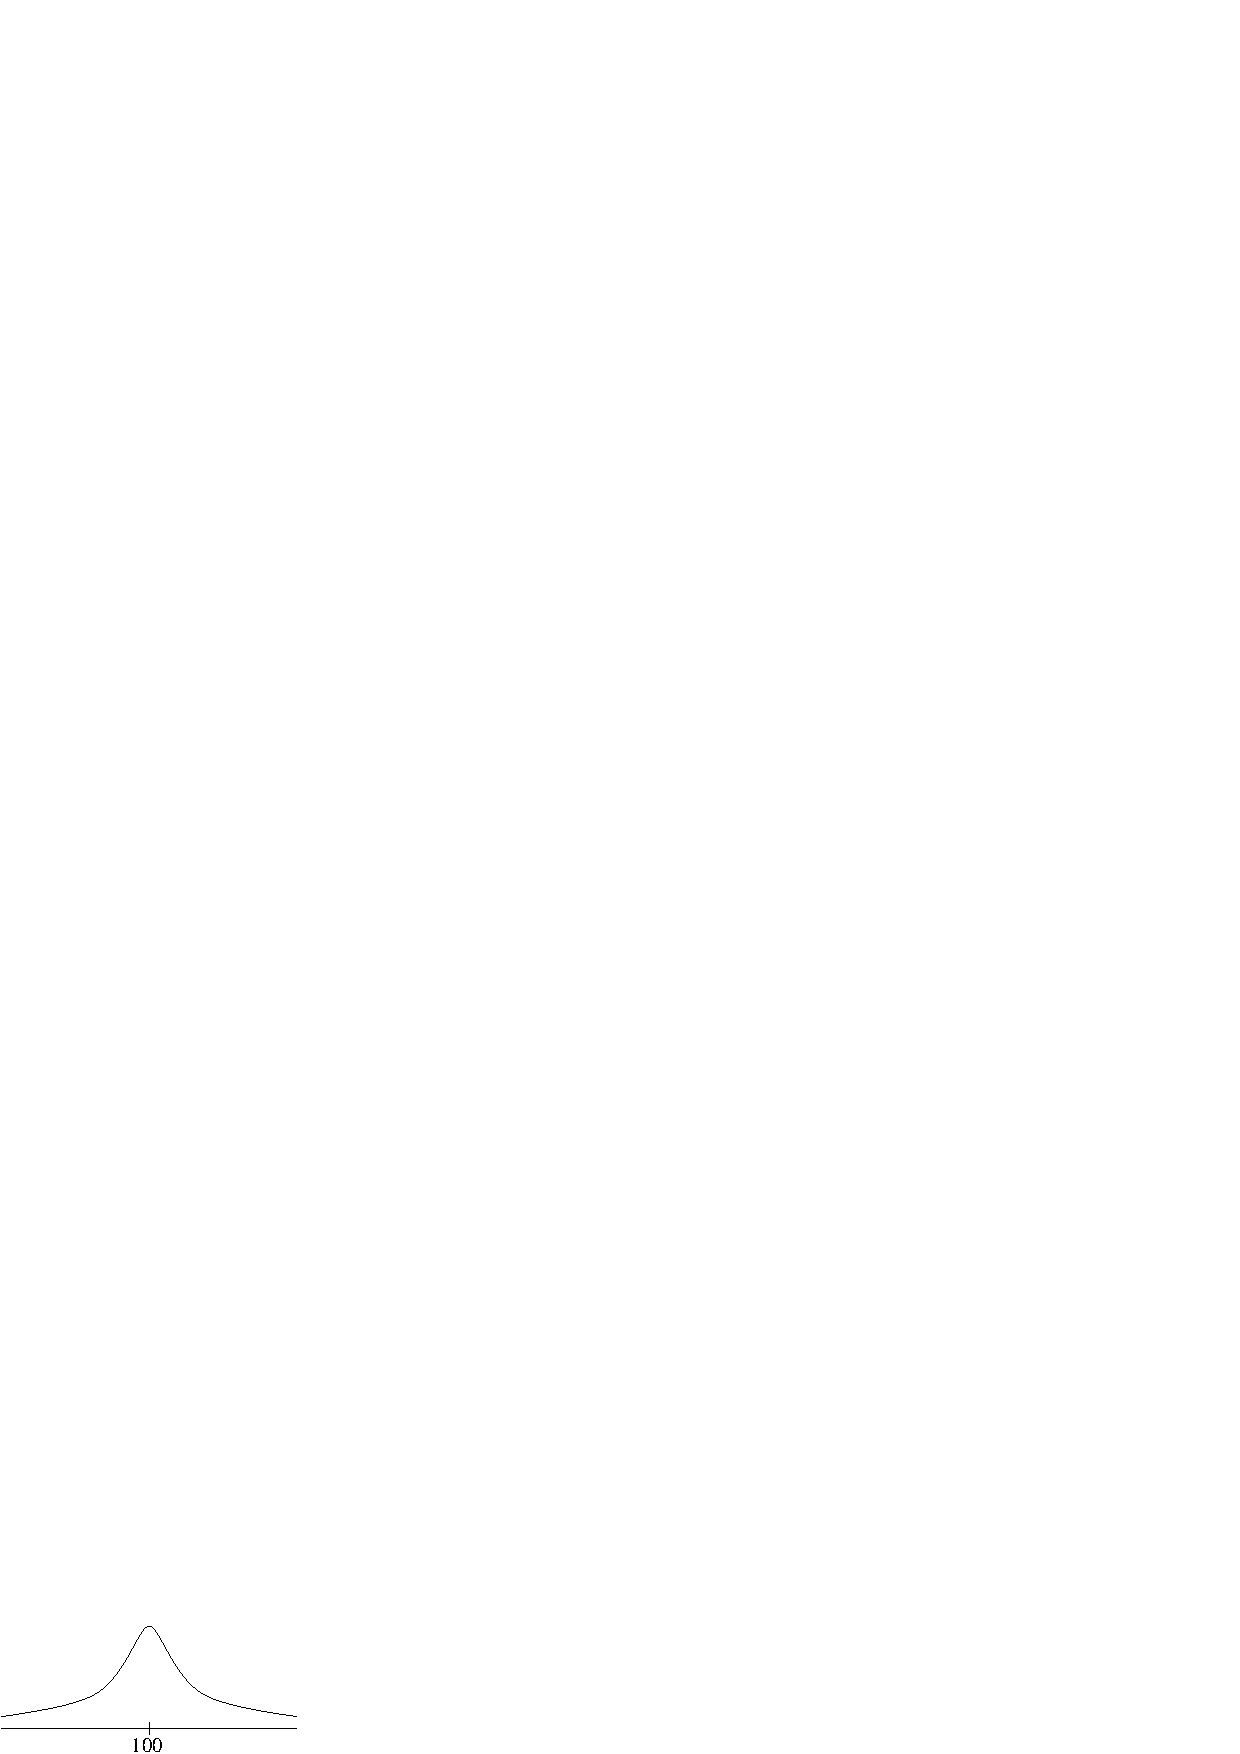
\includegraphics[width=2in]{figs/spread2.pdf}
\hskip.5in
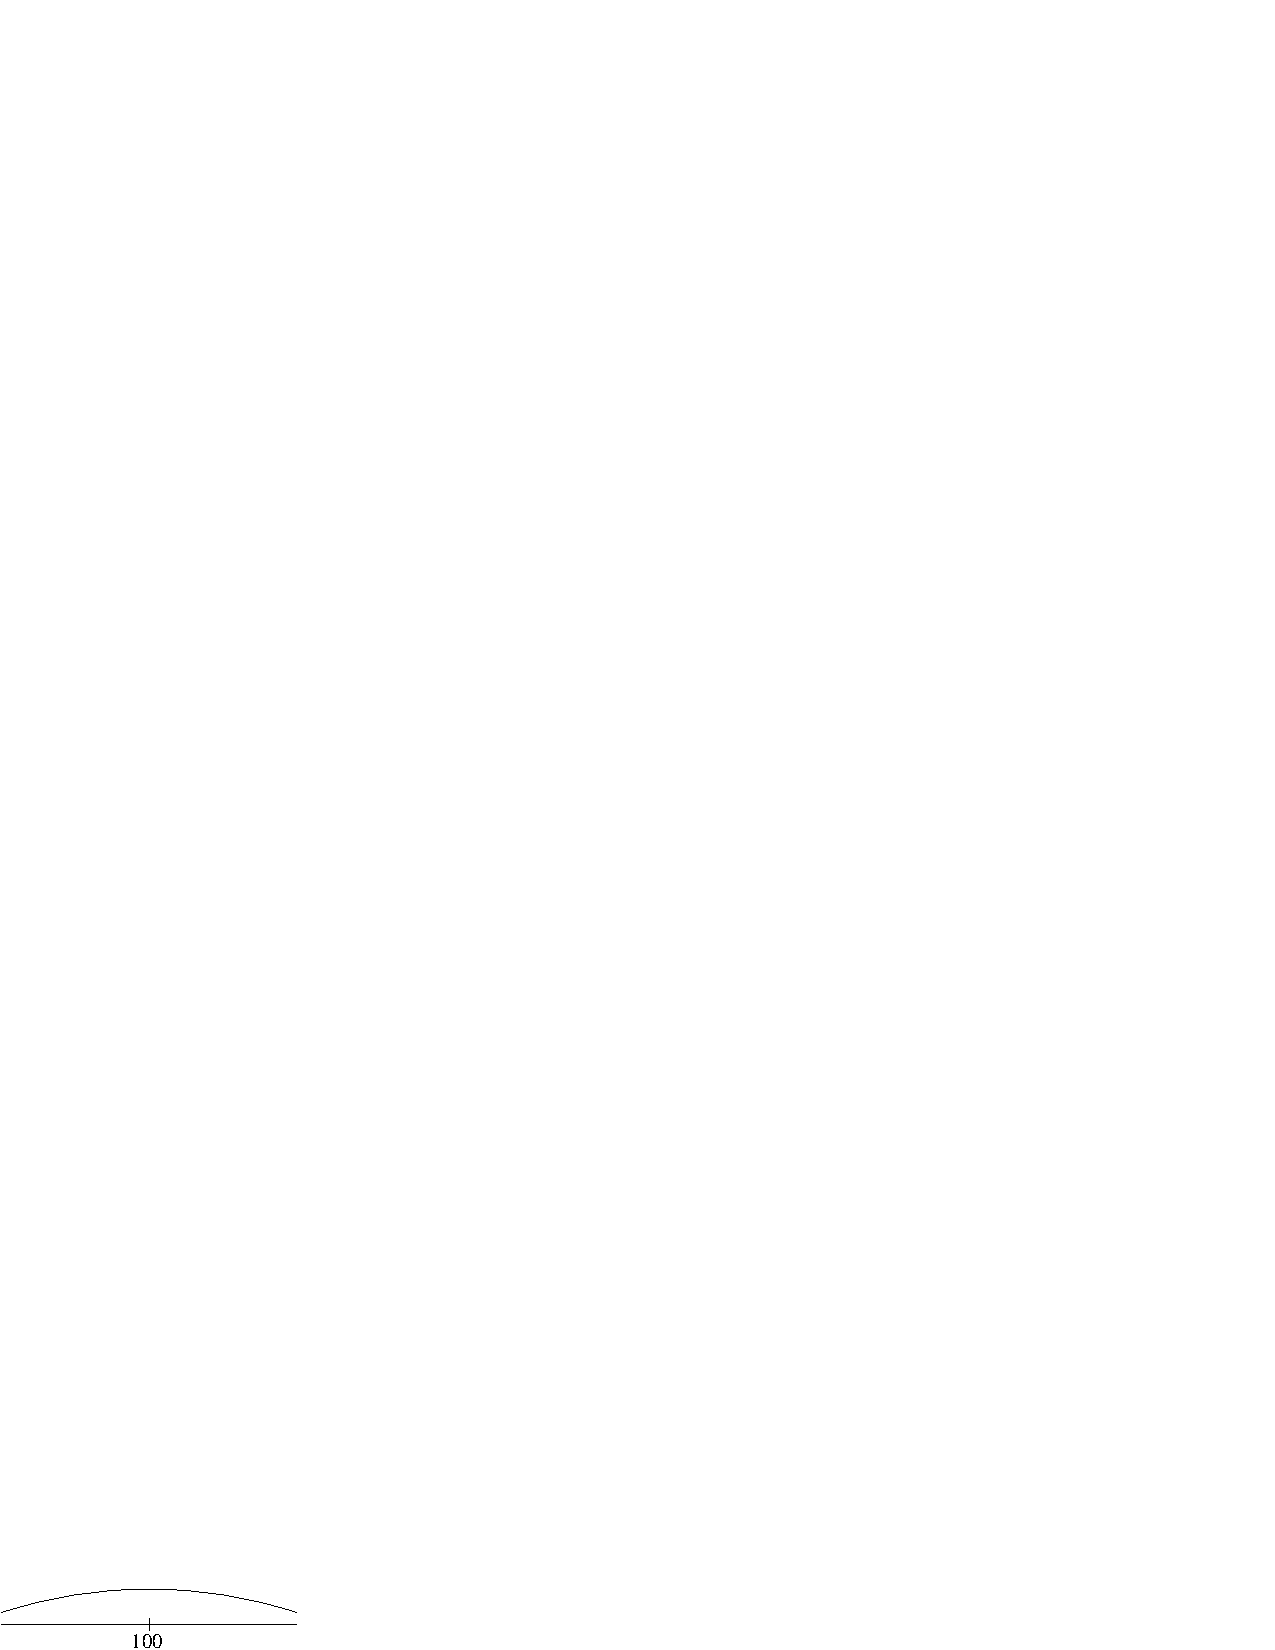
\includegraphics[width=2in]{figs/spread1.pdf}
\end{center}

\noindent
They both have the same expectation, 100, but one is concentrated near the middle 
while the other is pretty flat. To distinguish between them, we are interested
not just in the mean $\mu = \E(X)$, but also in the typical distance from the
mean, $\E(|X - \mu|)$. It turns out to be mathematically convenient to work with
the square instead: the {\it variance} of $X$ is defined to be
$$ \var(X)  \ = \ \E((X - \mu)^2) \ = \ \E((X - E(X))^2) .$$
In the above example, the distribution on the right has a higher variance that the
one on the left.

\subsection{Properties of the variance}

In what follows, take $\mu$ to be $\E(X)$.
\begin{enumerate}
\item The variance cannot be negative.

Since each individual value $(X - \mu)^2$ is $\geq 0$ (since its squared), the 
average value $\E((X - \mu)^2)$ must be $\geq 0$ as well.

\item $\var(X) = \E(X^2) - \mu^2$.

This is because
\begin{eqnarray*}
\var(X)  & = & \E((X - \mu)^2) \\
         & = & \E(X^2 + \mu^2 - 2\mu X) \\
         & = & \E(X^2) + \E(\mu^2) + \E(-2 \mu X) \ \ \mbox{(linearity)} \\
         & = & \E(X^2) + \mu^2 - 2 \mu \E(X) \\
         & = & \E(X^2) + \mu^2 - 2 \mu^2 \ = \ \E(X^2) - \mu^2.
\end{eqnarray*}

\item For any random variable $X$, it must be the case that $\E(X^2) \geq (\E(X))^2$.

This is simply because $\var(X) = \E(X^2) - (\E(X))^2 \geq 0$.

\item $\E(|X - \mu|) \leq \sqrt{\var(X)}$.

If you apply the previous property to the random variable $|X - \mu|$ instead of $X$,
you get $\E(|X - \mu|^2) \geq (\E(|X - \mu|))^2$. Therefore,
$\E(|X - \mu|) \leq \sqrt{\E(|X - \mu|^2)} = \sqrt{\var(X)}$. 
\end{enumerate}

The last property tells us that $\sqrt{\var(X)}$ is a good measure of the typical spread of
$X$: how far it typically lies from its mean. We call this the {\it standard deviation} of 
$X$.

\subsection{Examples}

\begin{enumerate}
\item Suppose you toss a coin with bias $p$, and let $X$ be $1$ if the outcome is heads, or 
$0$ if the outcome is tails.

Let's look at the distribution of $X$ and of $X^2$.

\begin{center}
\begin{tabular}{l|l|l}
Prob  & $X$ & $X^2$ \\ \hline
$p$   &  1  & 1     \\
$1-p$ &  0  & 0     
\end{tabular}
\end{center}

\noindent
From this table, $\E(X) = p$ and $\E(X^2) = p$. Thus the variance is 
$\var(X) = \E(X^2) - (\E(X))^2 = p(1-p)$.

\item Roll a 4-sided die (a tetrahedron) in which each face is equally likely to come
up, and let the outcome be $X \in \{1,2,3,4\}$.

We have two formulas for the variance: 
\begin{eqnarray*}
\var(X) & = & \E \left( (X - \mu)^2 \right) \\
\var(X) & = & \E(X^2) - \mu^2 
\end{eqnarray*}
where $\mu = \E(X)$.
Let's try both and make sure we get the same answer.
First of all, $\mu = \E(X) = (1 + 2 + 3 + 4)/4 = 2.5$. Now, let's tabulate the
distribution of $X^2$ and $(X-\mu)^2$.

\begin{center}
\begin{tabular}{l|l|l|l}
Prob  & $X$ & $X^2$ & $(X-\mu)^2$ \\ \hline
$1/4$ &  1  & 1     &  2.25 \\
$1/4$ &  2  & 4     &  0.25 \\
$1/4$ &  3  & 9     &  0.25 \\
$1/4$ &  4  & 16    &  2.25
\end{tabular}
\end{center}

\noindent
Reading from this table,
\begin{eqnarray*}
\E(X^2)     & = & \frac{1}{4} \left( 1 + 4 + 9 + 16 \right) \ \ = \ \ 7.5 \\
\E(X-\mu)^2 & = & \frac{1}{4} \left( 2.25 + 0.25 + 0.25 + 2.25 \right) \ \ = \ \ 1.25
\end{eqnarray*}
The first formula for variance gives $\var(X) = \E(X-\mu)^2 = 1.25$. The second
formula gives $\var(X) = \E(X^2) - \mu^2 = 7.5 - (2.5)^2 = 1.25$, the same thing.

\item Roll a $k$-sided die in which each face is equally likely to come up. The outcome
is $X \in \{1,2,\ldots,k\}$.

The expected outcome is
$$
\E(X) 
\ = \ 
\frac{1 + 2 + \cdots + k}{k} 
\ = \ 
\frac{\frac{1}{2} k(k+1)}{k}
\ = \ 
\frac{k+1}{2},
$$
using a special formula for the sum of the first $k$ integers. There's another for
the sum of the first $k$ squares, from which
$$
\E(X^2) 
\ = \ 
\frac{1^2 + 2^2 + \cdots + k^2}{k}
\ = \ 
\frac{\frac{1}{6}k(k+1)(2k+1)}{k}
\ = \ 
\frac{(k+1)(2k+1)}{6}.
$$
Then
$$
\var(X)
\ = \ 
\E(X^2) - (\E(X))^2
\ = \ 
\frac{(k+1)(2k+1)}{6} - \frac{(k+1)^2}{4}
\ = \ 
\frac{k^2 - 1}{12}.
$$
The standard deviation is thus approximately $k/\sqrt{12}$.

\item $X$ is the number of fixed points of a random permutation of $(1,2,\ldots,n)$.

Proceeding as before, let $X_i$ be 1 if $i$ is a fixed point of the permutation, and
0 otherwise. Then $\E(X_i) = 1/n$. For $i \neq j$, the product $X_i X_j$ is 1 only 
if both $i$ and $j$ are fixed points, which occurs with probability $1/n(n-1)$ (why?).
Thus $\E(X_i X_j) = 1/n(n-1)$. 

Since $X$ is the sum of the individual $X_i$, we have $\E(X) = 1$ and
\begin{eqnarray*}
\E(X^2) & = &
\E((X_1 + \cdots + X_n)^2) \\
& = & 
\E \left(\sum_{i=1}^n X_i^2 + \sum_{i \neq j} X_i X_j \right) \\
& = & 
\sum_i \E(X_i^2) + \sum_{i \neq j} \E(X_iX_j) \\
& = & 
n \cdot \frac{1}{n} + n(n-1) \cdot \frac{1}{n(n-1)}
\ = \ 
2.
\end{eqnarray*}
Thus $\var(X) = \E(X^2) - (\E(X)^2) = 1$. This means that the number of fixed points
has mean 1 and variance 1: in short, it is quite unlikely to be very much larger than
1.
\end{enumerate}

\subsection{Another property of the variance}

Here's a cartoon picture of a well-behaved distribution with mean $\mu$ and 
standard deviation $\sigma$ (that is, $\mu = \E(X)$ and $\sigma^2 = \var(X)$).

\begin{center}
%%\resizebox{2in}{!}{\input{figs/var.pstex_t}}
\end{center}

\noindent
The standard deviation quantifies the {\it spread} of the distribution
whereas the mean specifies its {\it location}. If you increase all values of
$X$ by 10, then the distribution will shift to the right and the mean will 
increase by 10. But the spread of the distribution -- and thus the standard
deviation -- will remain unchanged.

On the other hand, if you double all values of $X$, then its distribution 
becomes twice as wide, and thus its standard deviation $\sigma$ is doubled. 
Which means that its variance, which is the square of the standard deviation,
gets multiplied by 4.

In summary, for any constants $a,b$:
$$ \var(aX+b) = a^2 \var(X) .$$
Contrast this with the mean: $\E(aX + b) = a \E(X) + b$.

\subsection{Linearity of variance}

If $X$ and $Y$ are independent random variables, then $\var(X+Y) = \var(X) + \var(Y)$.
More generally, if $X_1, \ldots, X_n$ are independent, then
$$ \var(X_1 + \cdots + X_n)
\ = \ 
\var(X_1) + \cdots + \var(X_n).
$$
In contrast, linearity of expectation ($\E(X+Y) = \E(X) + \E(Y)$) holds
even if the random variables are {\it not} independent.


